\section{Waveform Groups}

A waveform group is a collection of one or more waveforms stacked vertically under a common timeline. All waveforms
within a group share the same timeline and vertical cursor(s).

When glscopeclient starts up, by default all channels on the attached instruments are displayed in a single waveform
group (Figure \ref{single-group}).

\begin{figure}[h]
\centering
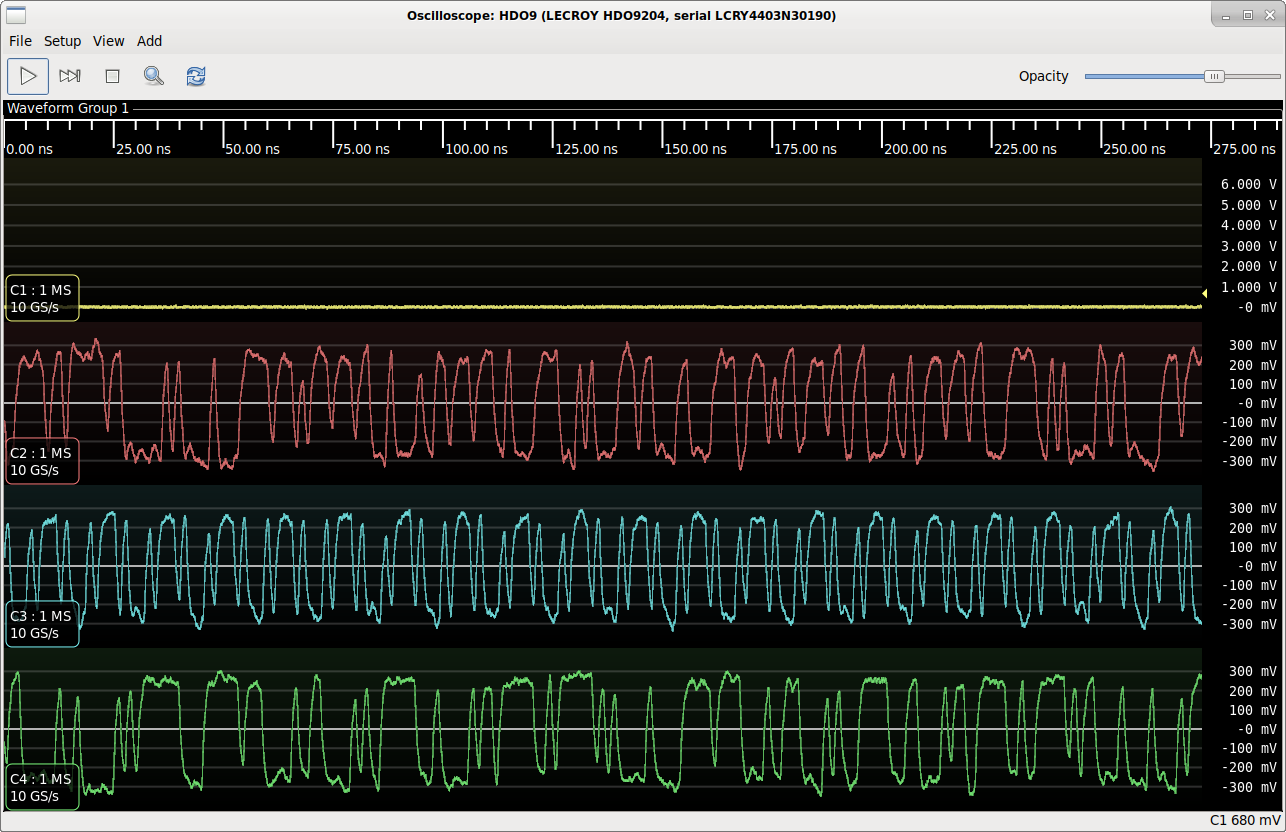
\includegraphics[width=13cm]{images/overview.png}
\caption{Top level glscopeclient window with a single waveform group}
\label{single-group}
\end{figure}

As you add protocol decodes or look at different parts of a waveform, it may be necessary to create additional waveform
groups. Typical reasons for creating additional groups include:

\begin{itemize}
\item Zooming into one set of signals to see detail on short time scales while maintaining a high level overview of
others
\item Viewing signals with incompatible horizontal units. For example, a FFT has horizontal units of frequency while an
analog waveform has horizontal units of time. Eye patterns also have horizontal units of time, but are always displayed
as two UIs wide and cannot be zoomed.
\footnote
{
It is currently possible to place signals with incompatible horizontal units in the same group. This may lead to
confusion; a future software release will likely force creation of a new group if a protocol decode is incompatible
with the parent trace's time scale.
}
\end{itemize}

\subsection{Managing Groups}

Additional groups may be created by right clicking a waveform and selecting \menustyle{[Move|Copy] waveform to / Insert
new group at [right|bottom]} from the context menu. This will split the current group's area in half horizontally or
vertically, with the selected waveform moved or copied to the newly added group and all other waveforms in the original
group.

Dividers between waveform groups may be dragged with the left mouse button. Any group may be subdivided again, to
create arbitrarily complex tiles of waveforms. Figure \ref{multiple-groups} shows a two-level hierarchy created by
moving channel 2 to a new group at right, moving channel 4 to this group, then moving channel 4 again a new group at
bottom.

\begin{figure}[h]
\centering
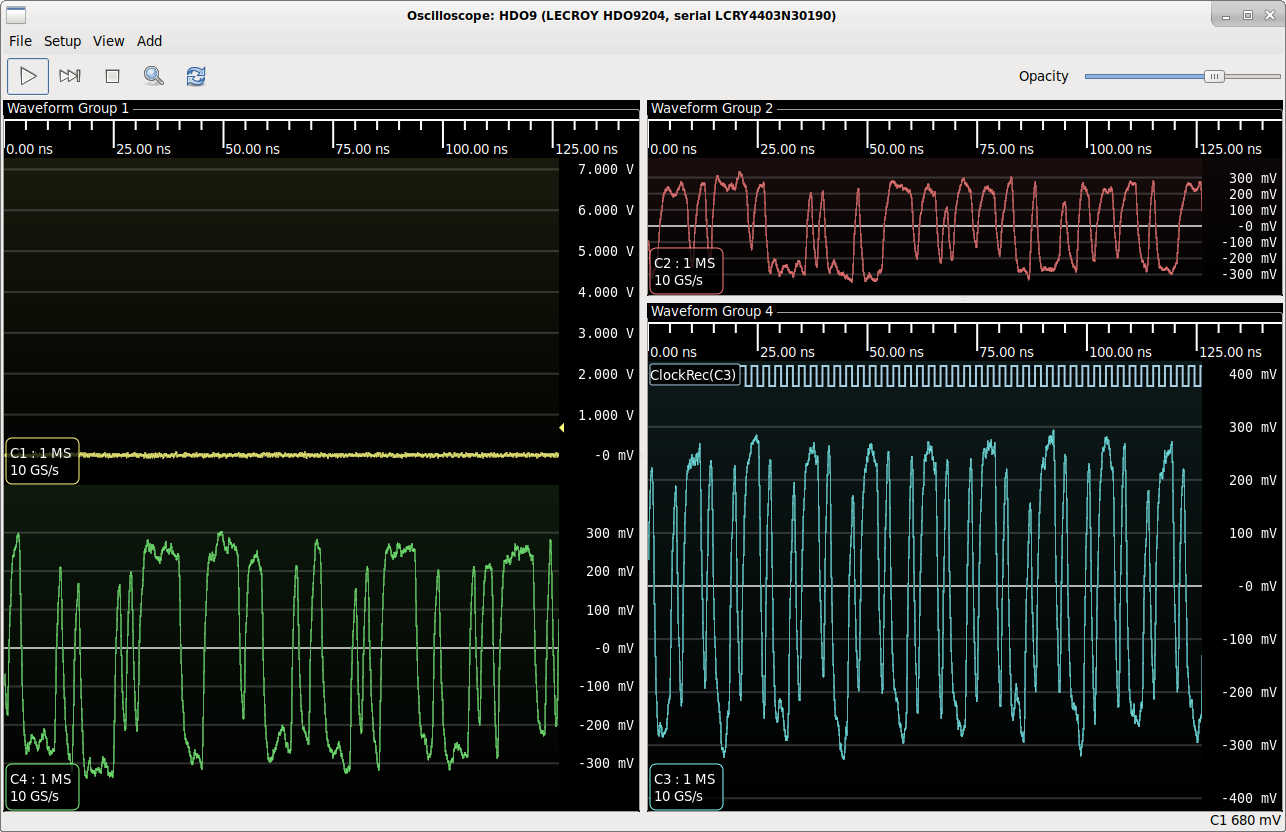
\includegraphics[width=14cm]{images/multiple-groups.png}
\caption{Top level glscopeclient window with several waveform groups separated by splitters}
\label{multiple-groups}
\end{figure}

A future software release will support using the mouse to move and copy waveforms, both between groups and within a
group (scopehal-apps:6). The exact semantics for this are not yet defined.

New waveform groups are given an automatically generated name when created, for example "Waveform Group 2". This name
will be editable in a future software release (scopehal-apps:53).

\pagebreak
\section{Timeline}

The timeline is displayed at the top of each waveform group and shows the X axis scale for the group. The timeline (and
all accompanying waveform views in the group) may be zoomed by scrolling with the mouse wheel, or panned by dragging
with the left mouse button.

Unlike classical oscilloscope user interfaces, there is \emph{no relationship} between the timeline scale/position and
the duration of the acquisition. It is possible to zoom or scroll beyond the end of the acquisition (displaying empty
background with no signal) or have a deep capture in which nearly all acquired data is offscreen.

TODO: talk about how to set trigger offset in capture and change timebase once that's implemented

TODO: insert screenshot after we have some pending UI changes done

\pagebreak
\section{Waveform Views}

A waveform view is a 2D graph of a signal or protocol decode within a waveform group.

\subsection{Plot Area}

The plot area shows the waveform being displayed. The background has a subtle gradient from light at top to dark at
bottom, in order to visually separate adjacent waveform view within the same group.

The horizontal grid lines line up with the voltage scale markings on the Y axis. If the plot area includes Y=0, the
grid line for zero is slightly brighter.

\begin{figure}[H]
\centering
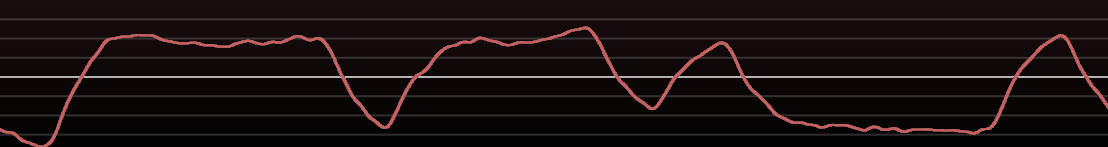
\includegraphics[width=10cm]{images/waveform-graph.png}
\caption{Waveform plot area}
\label{waveform-graph}
\end{figure}

The waveform is drawn as a semi-transparent line so that when zoomed out, the density of voltage at various points in
the graph may be seen as lighter or darker areas. This is referred to as ``intensity grading".

\begin{figure}[H]
\centering
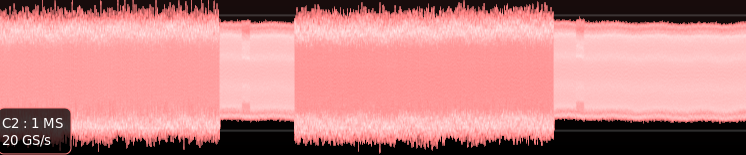
\includegraphics[width=10cm]{images/graded-waveform.png}
\caption{Intensity-graded waveform}
\label{graded-waveform2}
\end{figure}

\subsection{Y Axis Scale}

Each waveform view has its own Y axis scale, which is locked to the ADC range of the instrument.

Dragging the Y axis scale with the left mouse button currently does nothing (scopehal-apps:54) but in a future software
release will change the voltage offset of the channel.

Scrolling the Y axis scale with the mouse wheel changes the gain of the channel.

If a left-pointing arrow (as seen in Fig. \ref{y-axis}) is visible, the current channel is selected as a trigger
source. Click on the arrow and drag up or down to select the trigger level.

\begin{figure}[H]
\centering
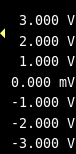
\includegraphics[height=3cm]{images/y-axis.png}
\caption{Y axis of a waveform view showing trigger arrow}
\label{y-axis}
\end{figure}

\subsection{Channel Information Box}

The channel information box is displayed in the lower left corner of each waveform view. It contains summary
information about the channel. Currently this is the display name of the channel, the sample rate, and the record
length of the acquisition. Other information, such as probe coupling, may be displayed there in the future.

Double-clicking the information box opens the channel properties dialog.

\begin{figure}[H]
\centering
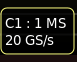
\includegraphics[width=2cm]{images/channel-infobox.png}
\caption{Channel information box}
\label{channel-infobox}
\end{figure}

\subsection{Overlays}

Waveforms may have additional information overlaid on top of them, such as protocol decodes. Each overlay has its own
information box, which may be double-clicked to open the properties dialog and configure it just like any other
channel.

Fig. \ref{overlays} shows
an example of an analog waveform with three overlays: thresholding it to NRZ digital, recovering a sampling
clock with a CDR PLL, and finally decoding the serial NRZ data stream to TMDS protocol data and control events.

\begin{figure}[H]
\centering
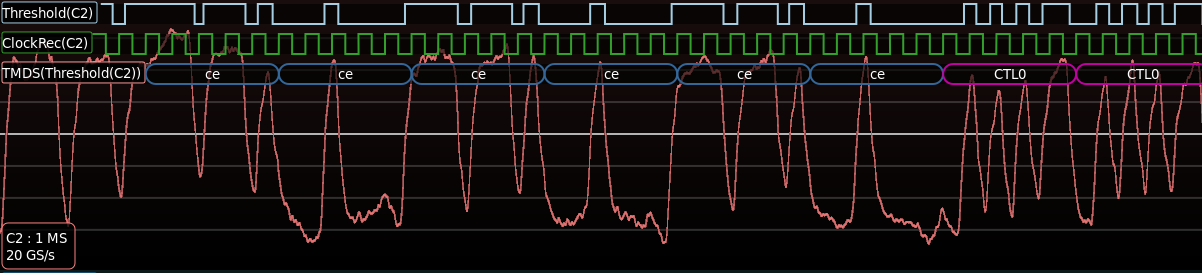
\includegraphics[width=14cm]{images/overlays.png}
\caption{Waveform showing two digital overlays and a data decode overlay}
\label{overlays}
\end{figure}

Overlays can be deleted but cannot currently be moved between waveform areas or reordered within a single waveform area
(scopehal-apps:7, scopehal-apps:6)
